
\documentclass{article} % For LaTeX2e
\usepackage{iclr2025_conference,times}

% Optional math commands from https://github.com/goodfeli/dlbook_notation.
%%%%% NEW MATH DEFINITIONS %%%%%

\usepackage{amsmath,amsfonts,bm}

% Mark sections of captions for referring to divisions of figures
\newcommand{\figleft}{{\em (Left)}}
\newcommand{\figcenter}{{\em (Center)}}
\newcommand{\figright}{{\em (Right)}}
\newcommand{\figtop}{{\em (Top)}}
\newcommand{\figbottom}{{\em (Bottom)}}
\newcommand{\captiona}{{\em (a)}}
\newcommand{\captionb}{{\em (b)}}
\newcommand{\captionc}{{\em (c)}}
\newcommand{\captiond}{{\em (d)}}

% Highlight a newly defined term
\newcommand{\newterm}[1]{{\bf #1}}


% Figure reference, lower-case.
\def\figref#1{figure~\ref{#1}}
% Figure reference, capital. For start of sentence
\def\Figref#1{Figure~\ref{#1}}
\def\twofigref#1#2{figures \ref{#1} and \ref{#2}}
\def\quadfigref#1#2#3#4{figures \ref{#1}, \ref{#2}, \ref{#3} and \ref{#4}}
% Section reference, lower-case.
\def\secref#1{section~\ref{#1}}
% Section reference, capital.
\def\Secref#1{Section~\ref{#1}}
% Reference to two sections.
\def\twosecrefs#1#2{sections \ref{#1} and \ref{#2}}
% Reference to three sections.
\def\secrefs#1#2#3{sections \ref{#1}, \ref{#2} and \ref{#3}}
% Reference to an equation, lower-case.
\def\eqref#1{equation~\ref{#1}}
% Reference to an equation, upper case
\def\Eqref#1{Equation~\ref{#1}}
% A raw reference to an equation---avoid using if possible
\def\plaineqref#1{\ref{#1}}
% Reference to a chapter, lower-case.
\def\chapref#1{chapter~\ref{#1}}
% Reference to an equation, upper case.
\def\Chapref#1{Chapter~\ref{#1}}
% Reference to a range of chapters
\def\rangechapref#1#2{chapters\ref{#1}--\ref{#2}}
% Reference to an algorithm, lower-case.
\def\algref#1{algorithm~\ref{#1}}
% Reference to an algorithm, upper case.
\def\Algref#1{Algorithm~\ref{#1}}
\def\twoalgref#1#2{algorithms \ref{#1} and \ref{#2}}
\def\Twoalgref#1#2{Algorithms \ref{#1} and \ref{#2}}
% Reference to a part, lower case
\def\partref#1{part~\ref{#1}}
% Reference to a part, upper case
\def\Partref#1{Part~\ref{#1}}
\def\twopartref#1#2{parts \ref{#1} and \ref{#2}}

\def\ceil#1{\lceil #1 \rceil}
\def\floor#1{\lfloor #1 \rfloor}
\def\1{\bm{1}}
\newcommand{\train}{\mathcal{D}}
\newcommand{\valid}{\mathcal{D_{\mathrm{valid}}}}
\newcommand{\test}{\mathcal{D_{\mathrm{test}}}}

\def\eps{{\epsilon}}


% Random variables
\def\reta{{\textnormal{$\eta$}}}
\def\ra{{\textnormal{a}}}
\def\rb{{\textnormal{b}}}
\def\rc{{\textnormal{c}}}
\def\rd{{\textnormal{d}}}
\def\re{{\textnormal{e}}}
\def\rf{{\textnormal{f}}}
\def\rg{{\textnormal{g}}}
\def\rh{{\textnormal{h}}}
\def\ri{{\textnormal{i}}}
\def\rj{{\textnormal{j}}}
\def\rk{{\textnormal{k}}}
\def\rl{{\textnormal{l}}}
% rm is already a command, just don't name any random variables m
\def\rn{{\textnormal{n}}}
\def\ro{{\textnormal{o}}}
\def\rp{{\textnormal{p}}}
\def\rq{{\textnormal{q}}}
\def\rr{{\textnormal{r}}}
\def\rs{{\textnormal{s}}}
\def\rt{{\textnormal{t}}}
\def\ru{{\textnormal{u}}}
\def\rv{{\textnormal{v}}}
\def\rw{{\textnormal{w}}}
\def\rx{{\textnormal{x}}}
\def\ry{{\textnormal{y}}}
\def\rz{{\textnormal{z}}}

% Random vectors
\def\rvepsilon{{\mathbf{\epsilon}}}
\def\rvtheta{{\mathbf{\theta}}}
\def\rva{{\mathbf{a}}}
\def\rvb{{\mathbf{b}}}
\def\rvc{{\mathbf{c}}}
\def\rvd{{\mathbf{d}}}
\def\rve{{\mathbf{e}}}
\def\rvf{{\mathbf{f}}}
\def\rvg{{\mathbf{g}}}
\def\rvh{{\mathbf{h}}}
\def\rvu{{\mathbf{i}}}
\def\rvj{{\mathbf{j}}}
\def\rvk{{\mathbf{k}}}
\def\rvl{{\mathbf{l}}}
\def\rvm{{\mathbf{m}}}
\def\rvn{{\mathbf{n}}}
\def\rvo{{\mathbf{o}}}
\def\rvp{{\mathbf{p}}}
\def\rvq{{\mathbf{q}}}
\def\rvr{{\mathbf{r}}}
\def\rvs{{\mathbf{s}}}
\def\rvt{{\mathbf{t}}}
\def\rvu{{\mathbf{u}}}
\def\rvv{{\mathbf{v}}}
\def\rvw{{\mathbf{w}}}
\def\rvx{{\mathbf{x}}}
\def\rvy{{\mathbf{y}}}
\def\rvz{{\mathbf{z}}}

% Elements of random vectors
\def\erva{{\textnormal{a}}}
\def\ervb{{\textnormal{b}}}
\def\ervc{{\textnormal{c}}}
\def\ervd{{\textnormal{d}}}
\def\erve{{\textnormal{e}}}
\def\ervf{{\textnormal{f}}}
\def\ervg{{\textnormal{g}}}
\def\ervh{{\textnormal{h}}}
\def\ervi{{\textnormal{i}}}
\def\ervj{{\textnormal{j}}}
\def\ervk{{\textnormal{k}}}
\def\ervl{{\textnormal{l}}}
\def\ervm{{\textnormal{m}}}
\def\ervn{{\textnormal{n}}}
\def\ervo{{\textnormal{o}}}
\def\ervp{{\textnormal{p}}}
\def\ervq{{\textnormal{q}}}
\def\ervr{{\textnormal{r}}}
\def\ervs{{\textnormal{s}}}
\def\ervt{{\textnormal{t}}}
\def\ervu{{\textnormal{u}}}
\def\ervv{{\textnormal{v}}}
\def\ervw{{\textnormal{w}}}
\def\ervx{{\textnormal{x}}}
\def\ervy{{\textnormal{y}}}
\def\ervz{{\textnormal{z}}}

% Random matrices
\def\rmA{{\mathbf{A}}}
\def\rmB{{\mathbf{B}}}
\def\rmC{{\mathbf{C}}}
\def\rmD{{\mathbf{D}}}
\def\rmE{{\mathbf{E}}}
\def\rmF{{\mathbf{F}}}
\def\rmG{{\mathbf{G}}}
\def\rmH{{\mathbf{H}}}
\def\rmI{{\mathbf{I}}}
\def\rmJ{{\mathbf{J}}}
\def\rmK{{\mathbf{K}}}
\def\rmL{{\mathbf{L}}}
\def\rmM{{\mathbf{M}}}
\def\rmN{{\mathbf{N}}}
\def\rmO{{\mathbf{O}}}
\def\rmP{{\mathbf{P}}}
\def\rmQ{{\mathbf{Q}}}
\def\rmR{{\mathbf{R}}}
\def\rmS{{\mathbf{S}}}
\def\rmT{{\mathbf{T}}}
\def\rmU{{\mathbf{U}}}
\def\rmV{{\mathbf{V}}}
\def\rmW{{\mathbf{W}}}
\def\rmX{{\mathbf{X}}}
\def\rmY{{\mathbf{Y}}}
\def\rmZ{{\mathbf{Z}}}

% Elements of random matrices
\def\ermA{{\textnormal{A}}}
\def\ermB{{\textnormal{B}}}
\def\ermC{{\textnormal{C}}}
\def\ermD{{\textnormal{D}}}
\def\ermE{{\textnormal{E}}}
\def\ermF{{\textnormal{F}}}
\def\ermG{{\textnormal{G}}}
\def\ermH{{\textnormal{H}}}
\def\ermI{{\textnormal{I}}}
\def\ermJ{{\textnormal{J}}}
\def\ermK{{\textnormal{K}}}
\def\ermL{{\textnormal{L}}}
\def\ermM{{\textnormal{M}}}
\def\ermN{{\textnormal{N}}}
\def\ermO{{\textnormal{O}}}
\def\ermP{{\textnormal{P}}}
\def\ermQ{{\textnormal{Q}}}
\def\ermR{{\textnormal{R}}}
\def\ermS{{\textnormal{S}}}
\def\ermT{{\textnormal{T}}}
\def\ermU{{\textnormal{U}}}
\def\ermV{{\textnormal{V}}}
\def\ermW{{\textnormal{W}}}
\def\ermX{{\textnormal{X}}}
\def\ermY{{\textnormal{Y}}}
\def\ermZ{{\textnormal{Z}}}

% Vectors
\def\vzero{{\bm{0}}}
\def\vone{{\bm{1}}}
\def\vmu{{\bm{\mu}}}
\def\vtheta{{\bm{\theta}}}
\def\va{{\bm{a}}}
\def\vb{{\bm{b}}}
\def\vc{{\bm{c}}}
\def\vd{{\bm{d}}}
\def\ve{{\bm{e}}}
\def\vf{{\bm{f}}}
\def\vg{{\bm{g}}}
\def\vh{{\bm{h}}}
\def\vi{{\bm{i}}}
\def\vj{{\bm{j}}}
\def\vk{{\bm{k}}}
\def\vl{{\bm{l}}}
\def\vm{{\bm{m}}}
\def\vn{{\bm{n}}}
\def\vo{{\bm{o}}}
\def\vp{{\bm{p}}}
\def\vq{{\bm{q}}}
\def\vr{{\bm{r}}}
\def\vs{{\bm{s}}}
\def\vt{{\bm{t}}}
\def\vu{{\bm{u}}}
\def\vv{{\bm{v}}}
\def\vw{{\bm{w}}}
\def\vx{{\bm{x}}}
\def\vy{{\bm{y}}}
\def\vz{{\bm{z}}}

% Elements of vectors
\def\evalpha{{\alpha}}
\def\evbeta{{\beta}}
\def\evepsilon{{\epsilon}}
\def\evlambda{{\lambda}}
\def\evomega{{\omega}}
\def\evmu{{\mu}}
\def\evpsi{{\psi}}
\def\evsigma{{\sigma}}
\def\evtheta{{\theta}}
\def\eva{{a}}
\def\evb{{b}}
\def\evc{{c}}
\def\evd{{d}}
\def\eve{{e}}
\def\evf{{f}}
\def\evg{{g}}
\def\evh{{h}}
\def\evi{{i}}
\def\evj{{j}}
\def\evk{{k}}
\def\evl{{l}}
\def\evm{{m}}
\def\evn{{n}}
\def\evo{{o}}
\def\evp{{p}}
\def\evq{{q}}
\def\evr{{r}}
\def\evs{{s}}
\def\evt{{t}}
\def\evu{{u}}
\def\evv{{v}}
\def\evw{{w}}
\def\evx{{x}}
\def\evy{{y}}
\def\evz{{z}}

% Matrix
\def\mA{{\bm{A}}}
\def\mB{{\bm{B}}}
\def\mC{{\bm{C}}}
\def\mD{{\bm{D}}}
\def\mE{{\bm{E}}}
\def\mF{{\bm{F}}}
\def\mG{{\bm{G}}}
\def\mH{{\bm{H}}}
\def\mI{{\bm{I}}}
\def\mJ{{\bm{J}}}
\def\mK{{\bm{K}}}
\def\mL{{\bm{L}}}
\def\mM{{\bm{M}}}
\def\mN{{\bm{N}}}
\def\mO{{\bm{O}}}
\def\mP{{\bm{P}}}
\def\mQ{{\bm{Q}}}
\def\mR{{\bm{R}}}
\def\mS{{\bm{S}}}
\def\mT{{\bm{T}}}
\def\mU{{\bm{U}}}
\def\mV{{\bm{V}}}
\def\mW{{\bm{W}}}
\def\mX{{\bm{X}}}
\def\mY{{\bm{Y}}}
\def\mZ{{\bm{Z}}}
\def\mBeta{{\bm{\beta}}}
\def\mPhi{{\bm{\Phi}}}
\def\mLambda{{\bm{\Lambda}}}
\def\mSigma{{\bm{\Sigma}}}

% Tensor
\DeclareMathAlphabet{\mathsfit}{\encodingdefault}{\sfdefault}{m}{sl}
\SetMathAlphabet{\mathsfit}{bold}{\encodingdefault}{\sfdefault}{bx}{n}
\newcommand{\tens}[1]{\bm{\mathsfit{#1}}}
\def\tA{{\tens{A}}}
\def\tB{{\tens{B}}}
\def\tC{{\tens{C}}}
\def\tD{{\tens{D}}}
\def\tE{{\tens{E}}}
\def\tF{{\tens{F}}}
\def\tG{{\tens{G}}}
\def\tH{{\tens{H}}}
\def\tI{{\tens{I}}}
\def\tJ{{\tens{J}}}
\def\tK{{\tens{K}}}
\def\tL{{\tens{L}}}
\def\tM{{\tens{M}}}
\def\tN{{\tens{N}}}
\def\tO{{\tens{O}}}
\def\tP{{\tens{P}}}
\def\tQ{{\tens{Q}}}
\def\tR{{\tens{R}}}
\def\tS{{\tens{S}}}
\def\tT{{\tens{T}}}
\def\tU{{\tens{U}}}
\def\tV{{\tens{V}}}
\def\tW{{\tens{W}}}
\def\tX{{\tens{X}}}
\def\tY{{\tens{Y}}}
\def\tZ{{\tens{Z}}}


% Graph
\def\gA{{\mathcal{A}}}
\def\gB{{\mathcal{B}}}
\def\gC{{\mathcal{C}}}
\def\gD{{\mathcal{D}}}
\def\gE{{\mathcal{E}}}
\def\gF{{\mathcal{F}}}
\def\gG{{\mathcal{G}}}
\def\gH{{\mathcal{H}}}
\def\gI{{\mathcal{I}}}
\def\gJ{{\mathcal{J}}}
\def\gK{{\mathcal{K}}}
\def\gL{{\mathcal{L}}}
\def\gM{{\mathcal{M}}}
\def\gN{{\mathcal{N}}}
\def\gO{{\mathcal{O}}}
\def\gP{{\mathcal{P}}}
\def\gQ{{\mathcal{Q}}}
\def\gR{{\mathcal{R}}}
\def\gS{{\mathcal{S}}}
\def\gT{{\mathcal{T}}}
\def\gU{{\mathcal{U}}}
\def\gV{{\mathcal{V}}}
\def\gW{{\mathcal{W}}}
\def\gX{{\mathcal{X}}}
\def\gY{{\mathcal{Y}}}
\def\gZ{{\mathcal{Z}}}

% Sets
\def\sA{{\mathbb{A}}}
\def\sB{{\mathbb{B}}}
\def\sC{{\mathbb{C}}}
\def\sD{{\mathbb{D}}}
% Don't use a set called E, because this would be the same as our symbol
% for expectation.
\def\sF{{\mathbb{F}}}
\def\sG{{\mathbb{G}}}
\def\sH{{\mathbb{H}}}
\def\sI{{\mathbb{I}}}
\def\sJ{{\mathbb{J}}}
\def\sK{{\mathbb{K}}}
\def\sL{{\mathbb{L}}}
\def\sM{{\mathbb{M}}}
\def\sN{{\mathbb{N}}}
\def\sO{{\mathbb{O}}}
\def\sP{{\mathbb{P}}}
\def\sQ{{\mathbb{Q}}}
\def\sR{{\mathbb{R}}}
\def\sS{{\mathbb{S}}}
\def\sT{{\mathbb{T}}}
\def\sU{{\mathbb{U}}}
\def\sV{{\mathbb{V}}}
\def\sW{{\mathbb{W}}}
\def\sX{{\mathbb{X}}}
\def\sY{{\mathbb{Y}}}
\def\sZ{{\mathbb{Z}}}

% Entries of a matrix
\def\emLambda{{\Lambda}}
\def\emA{{A}}
\def\emB{{B}}
\def\emC{{C}}
\def\emD{{D}}
\def\emE{{E}}
\def\emF{{F}}
\def\emG{{G}}
\def\emH{{H}}
\def\emI{{I}}
\def\emJ{{J}}
\def\emK{{K}}
\def\emL{{L}}
\def\emM{{M}}
\def\emN{{N}}
\def\emO{{O}}
\def\emP{{P}}
\def\emQ{{Q}}
\def\emR{{R}}
\def\emS{{S}}
\def\emT{{T}}
\def\emU{{U}}
\def\emV{{V}}
\def\emW{{W}}
\def\emX{{X}}
\def\emY{{Y}}
\def\emZ{{Z}}
\def\emSigma{{\Sigma}}

% entries of a tensor
% Same font as tensor, without \bm wrapper
\newcommand{\etens}[1]{\mathsfit{#1}}
\def\etLambda{{\etens{\Lambda}}}
\def\etA{{\etens{A}}}
\def\etB{{\etens{B}}}
\def\etC{{\etens{C}}}
\def\etD{{\etens{D}}}
\def\etE{{\etens{E}}}
\def\etF{{\etens{F}}}
\def\etG{{\etens{G}}}
\def\etH{{\etens{H}}}
\def\etI{{\etens{I}}}
\def\etJ{{\etens{J}}}
\def\etK{{\etens{K}}}
\def\etL{{\etens{L}}}
\def\etM{{\etens{M}}}
\def\etN{{\etens{N}}}
\def\etO{{\etens{O}}}
\def\etP{{\etens{P}}}
\def\etQ{{\etens{Q}}}
\def\etR{{\etens{R}}}
\def\etS{{\etens{S}}}
\def\etT{{\etens{T}}}
\def\etU{{\etens{U}}}
\def\etV{{\etens{V}}}
\def\etW{{\etens{W}}}
\def\etX{{\etens{X}}}
\def\etY{{\etens{Y}}}
\def\etZ{{\etens{Z}}}

% The true underlying data generating distribution
\newcommand{\pdata}{p_{\rm{data}}}
% The empirical distribution defined by the training set
\newcommand{\ptrain}{\hat{p}_{\rm{data}}}
\newcommand{\Ptrain}{\hat{P}_{\rm{data}}}
% The model distribution
\newcommand{\pmodel}{p_{\rm{model}}}
\newcommand{\Pmodel}{P_{\rm{model}}}
\newcommand{\ptildemodel}{\tilde{p}_{\rm{model}}}
% Stochastic autoencoder distributions
\newcommand{\pencode}{p_{\rm{encoder}}}
\newcommand{\pdecode}{p_{\rm{decoder}}}
\newcommand{\precons}{p_{\rm{reconstruct}}}

\newcommand{\laplace}{\mathrm{Laplace}} % Laplace distribution

\newcommand{\E}{\mathbb{E}}
\newcommand{\Ls}{\mathcal{L}}
\newcommand{\R}{\mathbb{R}}
\newcommand{\emp}{\tilde{p}}
\newcommand{\lr}{\alpha}
\newcommand{\reg}{\lambda}
\newcommand{\rect}{\mathrm{rectifier}}
\newcommand{\softmax}{\mathrm{softmax}}
\newcommand{\sigmoid}{\sigma}
\newcommand{\softplus}{\zeta}
\newcommand{\KL}{D_{\mathrm{KL}}}
\newcommand{\Var}{\mathrm{Var}}
\newcommand{\standarderror}{\mathrm{SE}}
\newcommand{\Cov}{\mathrm{Cov}}
% Wolfram Mathworld says $L^2$ is for function spaces and $\ell^2$ is for vectors
% But then they seem to use $L^2$ for vectors throughout the site, and so does
% wikipedia.
\newcommand{\normlzero}{L^0}
\newcommand{\normlone}{L^1}
\newcommand{\normltwo}{L^2}
\newcommand{\normlp}{L^p}
\newcommand{\normmax}{L^\infty}

\newcommand{\parents}{Pa} % See usage in notation.tex. Chosen to match Daphne's book.

\DeclareMathOperator*{\argmax}{arg\,max}
\DeclareMathOperator*{\argmin}{arg\,min}

\DeclareMathOperator{\sign}{sign}
\DeclareMathOperator{\Tr}{Tr}
\let\ab\allowbreak


\usepackage{hyperref}
\usepackage{tcolorbox}
\usepackage{tikz}
\usetikzlibrary{shapes.geometric, arrows}
\usetikzlibrary{shapes.geometric, arrows.meta, positioning}
\usepackage{url}
\usepackage{mdframed}


\usepackage{xcolor,listings}


\title{Lean-ing on Quality: \\ How High-Quality Data Beats Diverse Multilingual Data in AutoFormalization}

% Authors must not appear in the submitted version. They should be hidden
% as long as the \iclrfinalcopy macro remains commented out below.
% Non-anonymous submissions will be rejected without review.

% Willy Chan, Michael Souliman, Jakob Nordhagen
\author{%
  \textbf{Willy Chan}, \textbf{Michael Souliman}, \textbf{Jakob Nordhagen}, \textbf{Brando Miranda}, \textbf{Elyas Obbad}\\
  \textbf{Kai Fronsdal},
  \textbf{Sanmi Koyejo}\\
  \texttt{\{willyc, brando9\}@cs.stanford.edu} \\
  \textsuperscript{1}Department of Computer Science, Stanford University\\
}

% The \author macro works with any number of authors. There are two commands
% used to separate the names and addresses of multiple authors: \And and \AND.
%
% Using \And between authors leaves it to \LaTeX{} to determine where to break
% the lines. Using \AND forces a linebreak at that point. So, if \LaTeX{}
% puts 3 of 4 authors names on the first line, and the last on the second
% line, try using \AND instead of \And before the third author name.

\newcommand{\fix}{\marginpar{FIX}}
\newcommand{\new}{\marginpar{NEW}}

\iclrfinalcopy % Uncomment for camera-ready version, but NOT for submission.
\begin{document}


\maketitle

\begin{abstract}
% The abstract paragraph should be indented 1/2~inch (3~picas) on both left and
% right-hand margins. Use 10~point type, with a vertical spacing of 11~points.
% The word \textsc{Abstract} must be centered, in small caps, and in point size 12. Two
% line spaces precede the abstract. The abstract must be limited to one paragraph.

\textit{Autoformalization}, the translation of informal mathematics into formal Lean, is limited by the scarcity of paired formal-informal data. Backtranslation, in which a model informalizes formal text to create synthetic pairs, is established in machine translation and was applied to autoformalization by ProofNet (distilled backtranslation with GPT-4). We do not claim backtranslation as new. We compare four ways of generating paired data at a small scale: (1) on-the-fly (online) backtranslation, where one model informalizes and then re-formalizes a batch inside the training loop; (2) distilled backtranslation with a six-shot GPT-4 prompt over full Mathlib4 proofs; (3) informalization of each tactic together with the proof state before and after it, a step-level form of supervision related to process reward models; and (4) regular-expression templates. In the original submission, fine-tuning GPT-2 (124M parameters) on the six-shot GPT-4 data (71,550 tokens) gave a lower evaluation loss on the ProofNet test set than fine-tuning on the MMA dataset (10.9M tokens). In this revision we re-evaluate the released checkpoints and add MiniF2F, Lean-checked pass@$k$ (a sampled statement counts when Lean 4 with Mathlib compiles it), Gemma-2-2B and Llama-3-8B. The evaluation-loss ordering holds (3.30 vs 3.41) but the gap is smaller than first reported (3.12 vs 3.88), and the advantage of the six-shot data over MMA does not carry over to pass@$k$: for Gemma-2-2B it is higher on ProofNet pass@1 (+4.7 points) and lower on MiniF2F ($-4.0$ points), and for GPT-2 it is far lower on both. For Llama-3-8B, only on-the-fly backtranslation beats the 3-shot base model on ProofNet pass@16 (+6.4 points, 95\% interval [0.9, 12.0]). A compile check is also not a faithfulness check: the same pipeline accepts 94.5\% of gold statements taken from a different ProofNet task. We state what is still outside the scope of these results: other formal languages, human-in-the-loop data creation, and training seeds for the released checkpoints (see Limitations). We also report the cost of each generation method, examples of the generated data, and a check of every training set for overlap with ProofNet and MiniF2F.
\end{abstract}

\section{Introduction}
\noindent Neural machine translation has been a focal point of research since the early development of machine learning \citep{nmt2015baidu} \citep{nmt2016google}. \textit{Autoformalization} can be viewed as a specialized application of this approach, where the objective is to translate theorems from informal, human-readable markup languages like LaTeX into formal languages such as Lean4 --- a programming language specifically designed to encode complex mathematical constructs \citep{lean4}. In principle, the development of an agent capable of precise autoformalization would significantly reduce the prohibitive costs of manually formalizing proofs. This would have profound implications; such an advancement could render all mathematical knowledge, much of which is presently recorded in natural language, programmable: substantially enhancing the usability of interactive theorem proving systems and accelerating the expansion of human mathematical understanding \citep{klein2009formalization}.

Autoformalization first gained traction in 2018 when researchers used long short-term memory networks to generate statements in Mizar \citep{WangNMT}. More recently, experiments demonstrated promising results using a naive few-shot learning approach to translate English into Isabelle code \citep{autoformalization}.
% P.S. i have a bias for longer paragraphs, Can revert.
Historically, researchers have focused on merging automated theorem provers with language models, which often struggle with quantitative reasoning, limiting the types of theorems that can be expressed and solved and reducing the models' effectiveness in complex, real-world scenarios. We study one way of using interactive theorem provers with language models: fine-tuning a model on intermediary proof states from the LeanDojo dataset \citep{Leandojo}, paired with informal descriptions of each tactic, to test whether this step-level signal helps autoformalization. Step-level supervision of this kind is known from process reward models \citep{lightman2023lets,uesato2022solving}; our contribution is to apply it to informalization of Lean tactics and to measure it against other generation methods, not to introduce it.




While LLMs have performed well on benchmarks related to various natural language understanding tasks as evaluated by benchmarks such as MMLU \citep{MMLU}, they have continued to struggle with tasks that require deeper quantitative reasoning \citep{solvingQR}. Moreover, while strides have been made in using deep learning for symbolic mathematics \citep{DeepLearningSymbolic}, propositional logic \citep{TeachingLogics}, and differential systems \citep{LearningAMC}, the field of autoformalization and theorem proving has generally not seen proportional advances. This disparity can largely be attributed to two main factors:

\begin{enumerate}
    \item \textbf{Complexity: }Current models exhibit a gap in their ability to translate intricate mathematical concepts from natural language to formal logic.

    \item \textbf{Scarcity: }The available training data for fine-tuning models in formal languages like Lean is significantly limited. Given the specialized nature of these programming languages, the sum total of formal-math language data is a minuscule fraction of the size of modern LLMs' training datasets. Thus, except for hand-curated benchmarks such as ProofNet \citep{azerbayev2023proofnet} and MiniF2F \cite{minif2f}, there is virtually no paired formal-informal data.
\end{enumerate}

\begin{figure}[ht]
\centering
\begin{tcolorbox}[colframe=black!75!white, colback=white, boxrule=0.5mm, width=\linewidth, title={Example of Formal and Informal Statements}]
    \begin{minipage}{\linewidth}
    \textbf{Informal:} If $r$ is rational $(r \neq 0)$ and $x$ is irrational, prove that $r + x$ is irrational. \\
    \textbf{Formal:} theorem exercise\_1\_1a (x : R) (y : Q) : ( irrational x ) $\rightarrow$ irrational ( x + y ) := \\
    
    
    \textbf{Informal:} In an additive group $G$, the subtraction of vectors $g_1$ and $g_2$ is equal to the subtraction of the group elements $g_1$ and $g_2$. \\
    \textbf{Formal:} theorem vsub\_eq\_sub \{G : Type*\} [AddGroup G] (g\u2081 g\u2082 : G) : g\u2081 -\u1d65 g\u2082 = g\u2081 - g\u2082 :=   rfl \#align vsub\_eq\_sub vsub\_eq\_sub section General variable {G : Type*} {P : Type*} [AddGroup G] [T : AddTorsor G P]
    \end{minipage}
\end{tcolorbox}
\caption{\textbf{Autoformalization Task Example}. This table compares formal Lean statements with their equivalent informal mathematical statements. The formal statements represent theorems in Lean, while the informal statements convey the theorems in human-readable natural proof language.}

\label{fig:formal_informal_example}
\end{figure}


We present a new autoformalization dataset, \textbf{AI4Math}, which pairs statements from natural language proofs with their corresponding translations in Lean, as shown in Figure \ref{fig:formal_informal_example}. Our approach to generating this dataset leverages backtranslation: a method in neural machine translation for creating synthetic training data \citep{liu2021complementarity}. Given a monolingual dataset in the target language, backtranslation proceeds as follows:
\begin{enumerate}
    \item Utilize a pretrained model to generate translations in the reverse direction, i.e., from the target language to the source language.
    \item Assemble a parallel corpus consisting of these synthetic source and ground-truth target pairs.
    \item Fine-tune or train on the generated dataset, enabling the model to translate the synthetic source examples back to the target language.
\end{enumerate}

Our dataset, \textbf{AI4Math}, serves two primary purposes: first, to train an autoformalizer on individual statement pairs, and second, to fine-tune an LLM on the state of the proof before and after a specific tactic is applied. This approach aims to closely mimic the reasoning process in theorem proving, enhancing the LLM's ability to understand and generate formal proofs. 


Our \textbf{key contributions} are:
\begin{enumerate}
    \item A comparison of four generation methods for formal-informal pairs (on-the-fly backtranslation, distilled six-shot full-proof backtranslation, tactic-level informalization with proof states, and regular-expression templates) under one fine-tuning recipe, with their token counts and estimated API cost (Table~\ref{table:cost}) and examples of each (Figure~\ref{fig:examples}).

    \item Evidence, for GPT-2 (124M) and the ProofNet test set, that a small set of high-quality pairs (348 pairs, 71,550 tokens) reaches a lower evaluation loss than the MMA dataset (84,679 pairs, 10.9M tokens) \citep{mma}, re-evaluated in this revision with a smaller gap, and that tactic-level pairs with proof states improve on the pretrained baseline with 1,754 tokens.

    \item New in this revision: Lean-checked pass@$k$ on ProofNet and MiniF2F for GPT-2, Gemma-2-2B and Llama-3-8B (Section~\ref{sec:new}), which shows that the evaluation-loss advantage of the six-shot data over MMA does not appear consistently in pass@$k$, together with trust controls showing what a Lean compile does and does not measure.

    \item The AI4Math datasets and models, released on Hugging Face, with an overlap check of each training set against ProofNet and MiniF2F (Appendix~\ref{app:contamination}).
\end{enumerate}

\paragraph{What is not new.} Backtranslation for machine translation is due to \citet{sennrich-etal-2016-improving}. Distilled backtranslation for autoformalization, in which GPT-4 informalizes Mathlib statements and a smaller model is fine-tuned on the pairs, was introduced by ProofNet \citep{azerbayev2023proofnet}, and MMA \citep{mma} scaled it to a large multilingual set. Our six-shot full-proof method follows ProofNet's recipe with a different prompt. Supervising individual steps rather than final outcomes is the idea behind process reward models \citep{lightman2023lets,uesato2022solving}. What we add is the on-the-fly variant (one model plays both directions inside the training loop, with no teacher), the use of Lean proof states before and after each tactic as the context for informalization, and a controlled comparison of these methods against MMA at small token budgets.

\section{Training Data Generation via Backtranslation}

Backtranslation has been a pivotal method in neural machine translation (NMT), with its demonstrated utility for enhancing training efficacy in the absence of sufficient labeled data \citep{poncelas2018investigating}. This technique was further refined in transformer models \citep{han2021unsupervised} and in preliminary experiments involving distilled backtranslation within the domain of autoformalization \citep{azerbayev2023proofnet}. We chose this methodology because it is one of the most prominent and validated methods for NMT tasks \citep{liu2021complementarity}, and has been shown to be analytically and empirically suitable for neural model training \citep{mma}.


Our approach is to start with data in formal language (FL) and translate it into informal language (IL). We refer to this process as {\em informalization}. We compare the following generation methods, each of which we fine-tune on with the same recipe:

\begin{itemize}
\item \textbf{On-The-Fly Backtranslation: }This strategy for data augmentation utilized a unique backtranslation approach integrated within a custom training loop. Specifically, the training loop itself has four main steps, as outlined in Figure \ref{fig:on_the_fly_process}: (1) translating a batch of FL examples to IL (2) translating the synthetic IL examples back to FL, using the (synthetic IL, FL) pairs as labeled training data (3) computing the loss of the generated FL translations compared to the original FL examples and (4) backpropogating to update the model weights.

This method diverged from traditional practices by not employing separate teacher and student models; instead, it trained a single model to simultaneously manage both directions of the translation task. This setup was chosen because it enabled the model to iteratively generate its own training data at each step, and this self-sufficient nature allowed us to avoid the problem of limited labeled data without incurring large API costs. 

The relatively small size of the model used in our experiments, GPT-2 with 124M parameters, suggested that it would not be very effective at generating high-quality synthetic informalizations. Despite this, the on-the-fly backtranslation method led to a significant reduction in evaluation loss after just a few hundred training steps, eventually leading to a substantial improvement compared to the baseline as seen in Table \ref{table:model_loss}. Nevertheless, we eventually reached a performance plateau due to the inherent limitations of the baseline model. Due to resource constraints, we were unable to validate this method with a larger, more capable model such as Llemma-7B \citep{azerbayev2023llemma}. We hypothesize that employing a larger pretrained model could yield even more promising results. \label{methods:onthefly} This method thus serves as a baseline for comparison, and can highlight the potential benefits of using more powerful models in future work.

\begin{figure}[ht]
\centering
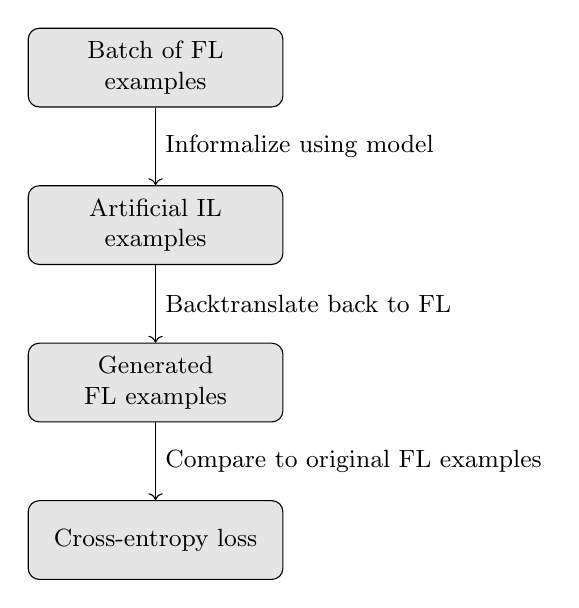
\begin{tikzpicture}[node distance=2.0cm, auto, font=\small]
    % Nodes
    \node[draw, rectangle, rounded corners, fill=gray!20, text width=3cm, minimum height=1cm, align=center] (fl) {Batch of FL examples};
    \node[draw, rectangle, rounded corners, fill=gray!20, below of=fl, text width=3cm, minimum height=1cm, align=center] (il) {Artificial IL examples};
    \node[draw, rectangle, rounded corners, fill=gray!20, below of=il, text width=3cm, minimum height=1cm, align=center] (gen_fl) {Generated FL examples};
    \node[draw, rectangle, rounded corners, fill=gray!20, below of=gen_fl, text width=3cm, minimum height=1cm, align=center] (loss) {Cross-entropy loss};

    % Edges
    \draw[->] (fl) to node[align=center] {Informalize using model} (il);
    \draw[->] (il) to node[align=center] {Backtranslate back to FL} (gen_fl);
    \draw[->] (gen_fl) to node[align=center] {Compare to original FL examples} (loss);
\end{tikzpicture}
\caption{\textbf{On-The-Fly Backtranslation Process Graph}. Given the scarcity of pairs of formal and informal mathematics, our solution is to generate artificial informal language (IL) translations from a formal language dataset (FL), then use the (IL, FL) pairs for training. This methodology first uses the LLM to translate from FL to IL, and then translates back to FL. This avoids the problem of lack of paired data by having the model generate training data on the fly to teach itself.}
\label{fig:on_the_fly_process}
\end{figure}

\item \textbf{Distilled Backtranslation:} Considering the limitations of our initial approach, we pivoted to a more robust technique known as \textit{distilled backtranslation}. For this method, we utilized a more powerful pretrained model, GPT-4 \citep{openai2023gpt4}, as the teacher model by feeding it a dataset of FL examples and utilizing it to generate corresponding synthetic IL text, as outlined in Figure \ref{fig:distilled_process}. We capitalized on the strong in-context learning capabilities of LLMs \citep{brown2020language} by employing a few-shot prompt that included six labeled examples of FL-to-IL translations. This few-shot amplification approach allowed us to develop a comprehensive labeled dataset for training, rather than generating data on-the-fly. The full technique and prompt can be found in \ref{fig:few_shot_prompt_example}, with a formal example in Appendix A.

Specifically, we extracted theorems from the MathLib4 dataset \citep{mathlib4} and then used GPT-4, enhanced by few-shot prompting, to informalize each theorem individually. Using regular expressions, we parsed over 100,000 theorems which we could later informalize and fine-tune on. However, due to the relatively high cost of using OpenAI's GPT-4 API, we were only able to informalize a small subset of these proofs as shown in Table \ref{table:dataset_composition}. Within this scope of distilled backtranslation, we compared several ways of looking at proofs:
\begin{enumerate}
    
    \item Our first method, inspired by techniques in \cite{azerbayev2023proofnet}, involves informalizing entire theorems while using the full proof as contextual support in the prompt, generating the theorem statement in natural language. We employed a 6-shot prompt to create a dataset of 348 training pairs for this approach.
    
     
    \item Our second method focuses on informalizing not only the theorem statement but also each individual tactic within a proof. This approach tests whether detailed explanations of each tactic can enhance the overall understanding of the proof. Utilizing the LeanDojo dataset \cite{Leandojo}, which is pre-parsed into distinct tactics, our prompts included the formal theorem statement and the states of the proof both before and after each tactic is applied. We employed a zero-shot prompting strategy with tuples of (stateBefore, tactic, stateAfter) to generate a dataset of individually translated tactics, aiming to improve translations between the complete Lean theorem and its natural language counterpart. \label{methods:indivLines}
\end{enumerate}

\item \textbf{Gathering Data from Regular Expressions:} We also prepared a large dataset leveraging only regular expressions for capturing specific lines/keywords in tactic scripts. Utilizing regular expressions for parsing LeanDojo proof tactics allowed us precise control over the selection of specific tactic lines and proof methodologies, enabling targeted improvements for specific areas of interest. An example of one of the filters we used to parse data from LeanDojo can be found in Figure \ref{figure:regular_expressions}. While these parsed informalizations are more rudimentary compared to our other methods, they allowed us to generate a much larger corpus at minimal cost. Additionally, this approach can be easily expanded upon and provides greater explainability than other methods. However, given the complexity of Lean code, this approach is inherently limited and can only produce rudimentary informalizations such as the ones in Appendix B. We hypothesized that while the model fine-tuned on Regex-parsed statements would enhance performance compared to the baseline, the simplicity of the translated statements would prevent them from outperforming more sophisticated backtranslation methods. This was confirmed by the results shown in Table \ref{table:model_loss}.
\end{itemize}


\begin{figure}[ht]
\centering
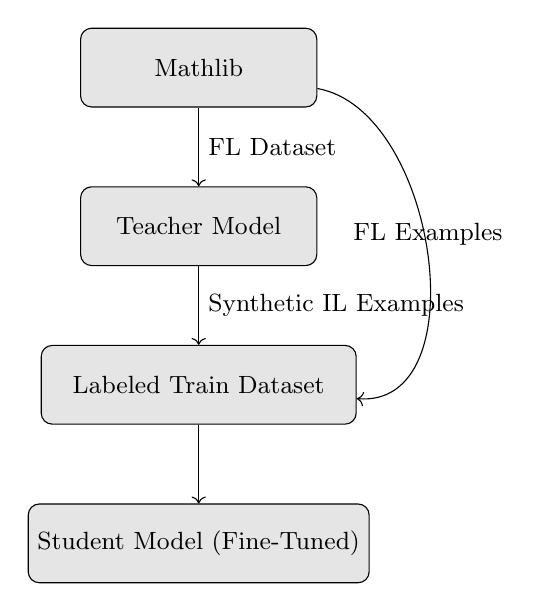
\begin{tikzpicture}[node distance=1.0cm, auto, font=\small]
    % Nodes
    \node[draw, rectangle, rounded corners, fill=gray!20, minimum width=3cm, minimum height=1cm, text centered] (mathlib) {Mathlib};
    \node[draw, rectangle, rounded corners, fill=gray!20, below=of mathlib, minimum width=3cm, minimum height=1cm, text centered] (teacher) {Teacher Model};
    \node[draw, rectangle, rounded corners, fill=gray!20, below=of teacher, minimum width=4cm, minimum height=1cm, text centered] (ltd) {Labeled Train Dataset};
    \node[draw, rectangle, rounded corners, fill=gray!20, below=of ltd, minimum width=4cm, minimum height=1cm, text centered] (student) {Student Model (Fine-Tuned)};

    % Edges
    \draw[->] (mathlib) -- (teacher) node[midway, right] {FL Dataset};
    \draw[->] (teacher) -- (ltd) node[midway, right] {Synthetic IL Examples};
    \draw[->] (ltd) -- (student) node[midway, right]{};
    
    % Skip connection
    \draw[->] (mathlib) to[out=350, in=-5] node[midway, above] {FL Examples} (ltd);

\end{tikzpicture}
\caption{\textbf{Distilled Backtranslation Process Graph}. Leveraging the MathLib and ProofNet datasets, a "Teacher" model translates formal theorems into synthetic informal language (IL) examples, which are then backtranslated to augment a training dataset with new formal language (FL) examples. A "Student" model, more compact than the teacher, is fine-tuned on this enriched dataset to improve its translation from IL to FL.}
\label{fig:distilled_process}
\end{figure}


\begin{figure}[ht]
\centering
\begin{tabular}{|l|}
\hline
\textbf{Regular Expressions} \\
\hline
\ttfamily patterns = \{ \\
\ \ \ \ "induction": r"induction .+ with .+", \\
\ \ \ \ "apply": r"apply .+", \\
\ \ \ \ "rewrite": r"rw .+", \\
\ \ \ \ "reflexivity": r"refl", \\
\ \ \ \ "cases": r"cases .+", \\
\ \ \ \ "introduce": r"intro .+|intros .+", \\
\ \ \ \ "simplification": r"simp .+", \\
\ \ \ \ "contradiction": r"contradiction", \\
\ \ \ \ "exact": r"exact .+", \\
\ \ \ \ "definition": r"def .+ := .+" \} \\
\hline
\end{tabular}
\caption{\textbf{Regular Expressions can be used to generate a large volume of rudimentary informalizations}. Certain Lean proof statements follow predictable patterns that can be captured via a regex. More sophisticated pattern-matching solutions can be built on this framework to increase the amount of paired data available to fine-tune on.}
\label{figure:regular_expressions}
\end{figure}


\section{AI4Math Dataset Overview}
The integration of data collected through these methodologies resulted in the \textbf{AI4Math} Dataset, which encompasses a broad spectrum of proof tactics and informal statements. The total number of tokens from each collection method is provided in Table \ref{table:dataset_composition}. The following datasets are labeled according to the composition of their contents:
\begin{enumerate}
    \item \textit{MMA Train} is a large, multilingual, and multi-domain baseline dataset \citep{mma} which we aim to compare our generated (IL, FL) pairs against. 
    
    \item \textit{On-the-Fly Backtranslation} is comprised of formal-informal pairs created as a result of the backtranslation procedure shown in Figure \ref{fig:formal_informal_example}.
    
    \item \textit{GPT-4 MathLib4 (Full Proof)} employs regular expressions to parse the MathLib4 dataset into individual theorems, using GPT-4 with few-shot prompting to informalize a selected subset. Following ProofNet's approach, we applied a 6-shot prompting technique to convert entire theorem statements and their proofs into natural language. This process is shown in Figure \ref{fig:distilled_process}.
        
    \item \textit{GPT-4 LeanDojo (Individual Tactics)} not only informalizes theorem statements but also each specific tactic within proofs from the LeanDojo dataset, capturing the proof's state before and after each tactic. Using a 0-shot prompting strategy, we created a dataset with informal translations of each tactic, alongside their respective before and after states.
    
    \item \textit{Regex-Parsed LeanDojo Proofs} uses regular expressions to parse specific tactics from the LeanDojo proofs for targeted model refinement. The filters used can be found in Appendix B.

\end{enumerate}


\begin{table}[ht]
\centering
\begin{tabular}{|l|c|}
\hline
\textbf{Data Collection Method} & \textbf{Token Count} \\
\hline
MMA Train &  10,916,097\\
\hline
Regex-Parsed LeanDojo Proofs & 124,782\\
\hline
GPT-4 MathLib4 (Full Proof) & 71,550\\
\hline
GPT-4 LeanDojo (Individual Tactics) & 1,754\\
\hline
% MiniF2F (Individual Tactics) & 23,761\\
% \hline
\end{tabular}
\caption{\textbf{Token counts across dataset generation methods}. For each dataset generation method, we compile formal and corresponding generated informal statement data into pairings. This illustrates the diversity and scale of training data available in AI4Math for fine-tuning, as well as demonstrating the relative cost of each synthetic dataset generation methodology.}
\label{table:dataset_composition}
\end{table}


\section{Examples of Generated Data}
Figure~\ref{fig:examples} shows one before/after pair per generation method, taken from the released data. Before is the formal Lean text; after is the informal text the method produced. The examples were drawn at random (seed 0) and cut to fit; five pairs per method are in \texttt{experiments/002\_examples\_cost\_datasets} of the project repository. On-the-fly backtranslation has no example: its synthetic informal text exists only inside the training loop and was not saved.

\begin{figure*}[htbp]
\centering
\begin{tabular}{|p{0.15\linewidth}|p{0.38\linewidth}|p{0.38\linewidth}|}
\hline
\textbf{Method} & \textbf{Before (formal)} & \textbf{After (informal)} \\
\hline
MMA Train (baseline) & \texttt{theorem refl\_trans (}$\alpha$\texttt{ : X }$\cong$\texttt{ Y) : Iso.refl X }$\ll\gg$ $\alpha$ \texttt{= }$\alpha$ \texttt{:=} & For any isomorphism '$\alpha$' from 'X' to 'Y', the composition of the identity isomorphism on 'X' and '$\alpha$' is equal to '$\alpha$'. \\
\hline
GPT-4 MathLib4 (Full Proof) & \texttt{theorem one\_le \{a : Associates }$\alpha$\texttt{\} : 1 }$\leq$\texttt{ a := Dvd.intro \_ (one\_mul a)} & For any associate $a$ of a type $\alpha$, $1$ is less than or equal to $a$. This is proven by introducing a divisor through the property that multiplying $1$ by $a$ gives $a$. \\
\hline
GPT-4 LeanDojo (Individual Tactics) & state before: $T \models \phi \leftrightarrow \exists T_0, T_0 \subseteq T \wedge T_0 \models \phi$; tactic: \texttt{simp only [models\_iff\_not\_satisfiable]}; state after: $\vdash \neg\,\mathrm{IsSatisfiable}(T \cup \{\neg\phi\}) \leftrightarrow \dots$ & In this scenario, we're dealing with a formal language $L$ and a theory $T$ within that language, [...] The goal is to prove the equivalence between $T$ proving $\phi$ and the existence of a subtheory $T_0$ of $T$ that also proves $\phi$. [...] \\
\hline
Regex-Parsed LeanDojo Proofs & \texttt{apply Nat.succ\_pos} & Here, we apply the theorem/lemma Nat.succ\_pos. \\
\hline
\end{tabular}
\caption{\textbf{Before/after examples for each generation method with saved data}. [...] marks text cut for space. Rows are from \texttt{AI4M/mma-dataset} (row 55125), \texttt{AI4M/gpt4-more} (row 183), \texttt{AI4M/state\_info\_informalization} (row 6) and \texttt{AI4M/regexInformalizationData} (row 601).}
\label{fig:examples}
\end{figure*}

\subsection{Cost of each generation method}
Table~\ref{table:cost} gives, for each method, the number of pairs, the GPT-2 token count, and an estimate of the GPT-4 API cost at OpenAI list prices (\$30 per million input tokens, \$60 per million output tokens). The dollar figures are estimates, not bills: no billing record or generation log survives, so they are lower bounds that count only the pairs we kept (calls that were dropped or retried are not logged), and wall-clock time was not recorded for any method. The MMA row is the price of regenerating its data with GPT-4; we did not pay it. The authors of MMA report \$3,500 for 332,000 informalized theorems \citep{mma}. The 1,754-token figure for the individual-tactics set in Table~\ref{table:dataset_composition} does not match either public individual-tactics set (29 pairs with 20,261 tokens; 100 pairs with 50,145 tokens); we report both.

\begin{table}[ht]
\centering
\small
\begin{tabular}{|p{0.30\linewidth}|r|r|r|}
\hline
\textbf{Method} & \textbf{Pairs} & \textbf{GPT-2 tokens} & \textbf{Est. API cost (USD)} \\
\hline
MMA Train (not paid by us) & 84,679 & 10,916,097 & 396 \\
\hline
GPT-4 MathLib4 (Full Proof) & 348 & 71,550 & $\geq$ 14 \\
\hline
GPT-4 LeanDojo (Individual Tactics), 29-pair set & 29 & 20,261 & $\geq$ 1 \\
\hline
GPT-4 LeanDojo (Individual Tactics), 100-pair set & 100 & 50,145 & $\geq$ 2 \\
\hline
Regex-Parsed LeanDojo Proofs & 2,875 & 124,782 & 0 (no API call) \\
\hline
On-the-Fly Backtranslation & not saved & not saved & 0 (GPU time only) \\
\hline
\end{tabular}
\caption{\textbf{Size and estimated GPT-4 cost of each generation method.} Estimates at list price, lower bounds, from \texttt{experiments/002\_examples\_cost\_datasets}. Wall-clock time was not logged. For the individual-tactics sets the zero-shot prompt text was not saved, so the input cost counts only the data.}
\label{table:cost}
\end{table}

\subsection{Overlap with the evaluation sets}
We checked every dataset in the Hugging Face organizations AI4M and UDACA (40 files from 33 repositories) for text overlap with the ProofNet and MiniF2F validation and test sets, by exact match and by at least 80\% shared 8-grams (Appendix~\ref{app:contamination}). The datasets used for the results in this paper are clean: MMA (train, validation, test), \texttt{gpt4-more} (the six-shot full-proof data), both individual-tactics sets and the regex sets have no overlapping item with ProofNet or MiniF2F. Several other released datasets do overlap, for example sets built from ProofNet itself and the data-selection sets built with ProofNet as the target; results from models trained on them must not be reported on ProofNet. This check is text matching only, on CPU, and does not show which data any given checkpoint was trained on.


\begin{figure*}[htbp]
\centering
\begin{mdframed}[linewidth=1pt, roundcorner=10pt, backgroundcolor=gray!10]
At the end of this explanation, I will give you 2 things. The first is a list of tuples that are the translations of entire proofs written in Lean, which we will denote the formal language, to plain English, also known as natural language, as tuples or pairs. This is not an exhaustive list, these are just examples of informalizations. I will then have a proof written in Lean represented as a string following the newline character after the list of pairs. Give me the tuple pair of the proof I give you written in Lean and what you think their natural language equivalent is given your knowledge of Lean, formatted using LaTeX. Do not output anything else, just the python tuple I requested. In your output match the exact format "('formal', 'informal')" \textbackslash n \\

\begin{verbatim}
[("Lean theorem statement 1", "Theorem 1 in natural language"),
("Lean theorem statement 2", "Theorem 2 in natural language"),
("Lean theorem statement 3", "Theorem 3 in natural language"),
("Lean theorem statement 4", "Theorem 4 in natural language"),
("Lean theorem statement 5", "Theorem 5 in natural language"),
("Lean theorem statement 6", "Theorem 6 in natural language")]
\end{verbatim}
\end{mdframed}
\caption{\textbf{Formal-informal pairs used for training are generated via few-shot prompting and distilled backtranslation}. Mined proofs from mathlib are used as input into this format string for prompting, and then GPT-4 creates examples that can be utilized for fine-tuning. In contrast to MMA, our method used six examples to informalize theorem statements.}
\label{fig:few_shot_prompt_example}
\end{figure*}


\section{Autoformalization Performance}


\begin{table}[ht]
\centering
\begin{tabular}{|l|c|c|}
\hline
\textbf{Fine-Tuning Dataset} & \textbf{Eval Loss, as first reported} & \textbf{Eval Loss, re-evaluated} \\
\hline
GPT-2 Baseline & 75.1839 & 3.81 \\
\hline
GPT-4 LeanDojo (Individual Tactics) & 5.1287 & not re-evaluated \\
\hline
Regex-Parsed LeanDojo Proofs & 4.4709 & not re-evaluated \\
\hline
On-the-Fly Backtranslation & 4.032 & not re-evaluated \\
\hline
MMA Train & 3.8791 & 3.41 \\
\hline
GPT-4 MathLib4 (Full Proof)& 3.1209 & 3.30 \\
\hline
\end{tabular}
\caption{\textbf{Evaluation loss on ProofNet's Test Dataset} (Lean 3 statements, whole-sequence cross-entropy). The model used was GPT-2, fine-tuned on each dataset for 3 epochs. The first column is the table of the original submission. The second column re-runs the paper's evaluation code on the released checkpoints (one checkpoint each, so there is no seed interval). The ordering of the three re-evaluated rows holds, the gap between the two datasets is 0.11 instead of 0.76, and the baseline of 75.18 does not reproduce (3.81; we did not find the cause). The four rows marked not re-evaluated keep their original values.}
\label{table:model_loss}
\end{table}

To quantify the results of our methods, we evaluate our fine-tuned models for accuracy on ProofNet's test dataset, with the goal of measuring the performance gain over their initial pretrained states. All of our models used GPT-2 as the base architecture and fine-tuned for 3 epochs using a learning rate of 1e-5 and Adafactor optimization, as these hyperparameters for the training setup appeared to yield the best performance. We chose GPT-2 for our experiments due to its open-source availability and lower fine-tuning costs compared to larger, closed-source models like GPT-4. As discussed, future research should consider using larger models to improve outcomes subject to resource availability.

We included the results of fine-tuning on the training set of MMA, a dataset that also uses GPT-4 to create the formal-informal pairs that matches the approach we took with the full-proof informalizations \citep{mma}. However, our methodology uses a 6-shot prompt only, which appears to improve token efficiency as evidenced by the lower token count in Table \ref{table:dataset_composition} and lower resulting evaluation loss in Table \ref{table:model_loss}.



We have three observations from the original GPT-2 evaluation-loss experiment; Section~\ref{sec:new} tests them with pass@$k$ and larger models.
\begin{itemize}
    \item \textbf{Few-Shot Beats MMA on GPT-2 evaluation loss, by a smaller margin than first reported}: Our \textit{GPT-4 MathLib4 (Full Proof)} dataset, developed through a hard-coded 6-shot prompting technique, reached a lower evaluation loss than the larger, diverse dataset from Albert et al., despite being over 150 times smaller (3.30 vs 3.41 on re-evaluation). The advantage sits in the natural-language tokens: on the formal tokens alone MMA is better (Section~\ref{sec:new}). We do not show that the informalizations are better, only that the loss is lower in this one setting.

    \item \textbf{Individual Tactics are Efficient}: The \textit{GPT-4 LeanDojo (Individual Tactics)} dataset, which leverages an intensive approach of matching individual tactics to lines in the informalized proof, demonstrated dramatic improvement from GPT-2 baseline with far fewer tokens compared to other methods. However, this method first requires having GPT-4 informalize the proof as a whole, and then pairing the individual tactics to a line in the translated natural language proof: making the strategy more costly at \$0.15 per proof compared to \$0.05 per proof in \textit{GPT-4 MathLib4 (Full Proof)} and the \$0.01 per proof in MMA, which had 332,000 theorems informalized for \$3,500 total \citep{mma}. This was the largest barrier preventing us from generating a larger training corpus. Given the drastic improvement compared to the baseline, we hypothesize that this is method has significant potential and should be explored in the future with more resources. 

    \item \textbf{On-The-Fly Backtranslation Performance Plateau}: When generating the distilled backtranslation dataset for the individual tactics, a review of the data showed that the model trained on our On-the-Fly Backtranslation dataset considerably outperformed the GPT-2 baseline, but its performance plateaued below that of the MMA dataset. We hypothesize that this is due to model size, as both of our best performing methodologies used GPT-4 to generate data for backtranslation.
\end{itemize}

\begin{tcolorbox}[colframe=blue, colback=white, boxrule=0.5mm, width=\linewidth, title={}]
    \textbf{Takeaway \#1: Few high-quality pairs can match a much larger set on evaluation loss, but the evidence is mixed on pass@$k$.} \\
    On GPT-2, \textit{GPT-4 MathLib4 (Full Proof)} reaches a lower evaluation loss than MMA with about 150 times fewer tokens. In Lean-checked pass@$k$ the comparison has no single sign: higher for Gemma-2-2B (5 epochs) on ProofNet, lower on MiniF2F, and far lower for GPT-2 (Section~\ref{sec:new}).
    \vspace{0.5em}

    \textbf{Takeaway \#2: Intermediate Steps Matter} \\
    \textit{GPT-4 Lean (Individual Tactics)} demonstrates remarkable proof-efficiency for the small token count despite the higher costs and poor performance compared to utilizing the full proof. 
    \vspace{0.001em}

    \textbf{Takeaway \#3: Data quality and diversity trade off by benchmark.} \\
    Richer GPT-4 prompts give a lower GPT-2 evaluation loss than MMA, but MMA has the higher pass@$k$ on MiniF2F for both Gemma-2-2B gpt4-more checkpoints, so the benchmark decides which dataset looks better. On Llama-3-8B, on-the-fly backtranslation, which uses no teacher, is the only fine-tune that beats the 3-shot base model on ProofNet pass@16.
    \vspace{0.5em}
\end{tcolorbox}


\section{Additional Experiments: Lean-Checked pass@$k$, MiniF2F and Larger Models}
\label{sec:new}
Reviewers asked for a second benchmark, a metric closer to use than evaluation loss, and models larger than GPT-2. This section reports those. All numbers here are from Lean-checked compilation or from cross-entropy on the released checkpoints; no language model judged any output. Sampling, training and cross-entropy ran on free university GPUs, and the Lean check ran on CPU.

\paragraph{Setup.} pass@$k$ is the share of tasks for which at least one of $k$ sampled Lean formalizations compiles (Lean 4.15 with Mathlib); it is computed from $n$ samples per task with the unbiased estimator. Compiling means the statement type-checks with \texttt{sorry} allowed as proof; it does not mean the statement is equal to the gold statement. We use the ProofNet test set (183 Lean 4 tasks) and MiniF2F test (244 Lean 4 tasks; the GPT-2 and Gemma experiment uses the 225 whose gold statement is not commented out, the Llama experiment uses all 244). For GPT-2 and Gemma-2-2B we use the released checkpoints (\texttt{AI4M} organization), $n=32$ samples, 3 sampling seeds (mean $\pm$ sd over seeds). The prompt format was chosen per model on ProofNet validation among 5 formats, so each model is compared at its own best prompt. For Llama-3-8B we fine-tune with LoRA (rank 64; not a full fine-tune) on gpt4-more, MMA (1 epoch, the original recipe uses 3) and on-the-fly backtranslation (2,000 MMA formal statements, because the LeanDojo corpus is not on Hugging Face), with $n=100$ samples and 1 sampling seed. TFA and TFCE are the teacher-forced token accuracy and cross-entropy on the formal tokens only.

\begin{table}[ht]
\centering
\small
\renewcommand{\arraystretch}{1.15}
\begin{tabular}{|l|r|r|r|r|r|r|}
\hline
\textbf{Model, fine-tuning data} & \multicolumn{2}{c|}{\textbf{ProofNet pass@$k$}} & \multicolumn{2}{c|}{\textbf{MiniF2F pass@$k$}} & \textbf{CE} & \textbf{TFA} \\
 & $k$=1 & $k$=32 & $k$=1 & $k$=32 & & \\
\hline
GPT-2, gpt4-more & 0.2 & 6.0 & 0.1 & 2.5 & 3.30 & 33.7 \\
GPT-2, MMA & 5.8 & 78.7 & 11.8 & 95.3 & 3.41 & 48.0 \\
\hline
Gemma-2-2B, none (3-shot) & 1.4 & 24.4 & 12.9 & 81.2 & 2.50 & 40.2 \\
Gemma-2-2B, gpt4-more 1 epoch & 6.0 & 67.0 & 12.9 & 96.4 & 2.23 & 56.1 \\
Gemma-2-2B, gpt4-more 5 epochs & 10.5 & 77.4 & 15.6 & 96.3 & 2.71 & 56.0 \\
Gemma-2-2B, MMA & 5.7 & 63.7 & 19.5 & 99.0 & 1.81 & 60.2 \\
\hline
\end{tabular}
\caption{\textbf{Lean-checked pass@$k$ (percent), GPT-2 and Gemma-2-2B.} Mean over 3 sampling seeds, 32 samples per task; sd over seeds is at most 0.6 at $k$=1 and 3.8 at $k$=32. CE and TFA (percent) are on ProofNet Lean 3 test (186 tasks), one released checkpoint each. Per-model intervals and pass@4 and pass@16 are in \texttt{experiments/03\_passk\_small\_models}. GPT-2 gpt4-more produces a theorem-shaped sample only 29\% of the time and ignored all 5 prompt formats tried, so its low pass@$k$ shows that the checkpoint does not follow a usable prompt.}
\label{table:passk_small}
\end{table}

\begin{table}[ht]
\centering
\small
\renewcommand{\arraystretch}{1.15}
\begin{tabular}{|l|r|r|r|r|}
\hline
\textbf{Llama-3-8B, 3-shot prompt} & \textbf{ProofNet pass@16} & \textbf{MiniF2F pass@16} & \textbf{TFA} & \textbf{CE} \\
\hline
base (no fine-tuning) & 41.4 & 98.2 & 57.3 & 1.97 \\
+ gpt4-more & 38.9 & 93.4 & 66.4 & 1.61 \\
+ MMA & 37.8 & 94.2 & 65.3 & 1.80 \\
+ on-the-fly backtranslation & 47.8 & 95.5 & 66.5 & 1.76 \\
\hline
\end{tabular}
\caption{\textbf{Llama-3-8B, Lean-checked pass@16 (percent), base against fine-tuned with the same 3 worked examples in the prompt.} ProofNet: 183 Lean 4 tasks; MiniF2F: 244. One sampling seed, 100 samples per task, LoRA rank 64. Rows prompted with the format each model was trained on are in \texttt{experiments/04\_llama3\_8b}; the base model scores 0.0 on that format because it never saw it. TFA and CE on ProofNet Lean 3 test.}
\label{table:passk_llama}
\end{table}

\paragraph{Trust controls: a compile is not a faithfulness check.} We ran the same wrap, rename and Lean check on gold statements. Gold compiles in 96.7\% of ProofNet tasks and 99.1\% of MiniF2F tasks; gold with one closing parenthesis deleted compiles in 0\% (the check rejects broken statements); and the gold statement of a different task compiles in 94.5\% of ProofNet tasks and 99.1\% of MiniF2F tasks (so the check accepts a wrong statement as long as it type-checks). Exact match with the gold statement is at most 0.3\% at pass@1. The pass@$k$ numbers therefore measure the rate of well-formed statements, not correct formalization, and we do not report them as accuracy.

\paragraph{Findings.}
\begin{itemize}
    \item \textbf{The GPT-2 evaluation-loss result does not reproduce in size.} Re-evaluating the released GPT-2 checkpoints gives CE 3.30 (gpt4-more), 3.41 (MMA) and 3.81 (base). The paper's slides gave 2.33 vs 2.69 and its table 3.12 vs 3.88 with a baseline of 75.18. The ordering holds; the gap is 0.11 here. On the formal tokens alone MMA is better (TFCE 3.03 vs 3.59, TFA 48.0\% vs 33.7\%, $p<0.001$), so the small CE advantage of gpt4-more sits in the natural-language tokens.
    \item \textbf{The gpt4-more vs MMA gap in pass@$k$ has no single sign} (paired over tasks, difference = gpt4-more minus MMA, sign-flip test). Gemma-2-2B with 5 epochs: ProofNet pass@1 $+4.7$ points [3.2, 6.3], MiniF2F pass@1 $-4.0$ [$-5.6$, $-2.4$]. Gemma-2-2B with 1 epoch: ProofNet $+0.3$ ($p=0.60$), MiniF2F $-6.6$ ($p<0.001$). GPT-2: $-5.6$ on ProofNet and $-11.8$ on MiniF2F, with the prompt-following caveat in Table~\ref{table:passk_small}.
    \item \textbf{Fine-tuning helps small models and gives little to Llama-3-8B on pass@$k$.} TFA gains are +8.5 to +22.8 points for GPT-2, +16 to +20 for Gemma-2-2B and +8 to +9 for Llama-3-8B. ProofNet pass@16 gains over the 3-shot base are +31 to +48 points for Gemma-2-2B but at most +6.4 for Llama-3-8B, whose base is already strong (41.4\% on ProofNet and 98.2\% on MiniF2F, against 15.6\% and 67.7\% for Gemma). For Llama-3-8B, on-the-fly backtranslation is the only fine-tune above the base on ProofNet pass@16: $+6.4$ points [0.9, 12.0]; gpt4-more ($-2.4$) and MMA ($-3.6$) are within noise, and on MiniF2F every fine-tune is 2.7 to 4.7 points below the base.
    \item \textbf{Which tasks.} For Gemma-2-2B 5 epochs, ProofNet pass@1 is highest on Artin, Dummit-Foote and Herstein (17.6, 14.3 and 19.4\%, against 6.9, 5.5 and 5.8\% for MMA); MMA leads on Pugh and on every MiniF2F family except algebra. Rudin, Munkres and Axler are the hardest for all models (pass@1 at most 6.6\%).
\end{itemize}
These results use one released checkpoint per setting (no training seeds), so differences between datasets are measured against sampling and task variation only, not training variation.

\section{Related Work}
The closest prior work is ProofNet \citep{azerbayev2023proofnet}, which introduced distilled backtranslation for autoformalization (GPT-4 informalizes Mathlib statements, a smaller model is fine-tuned on the pairs), and MMA \citep{mma}, which applied zero-shot GPT-4 informalization at scale across several formal languages. Our six-shot full-proof data is a variant of ProofNet's recipe, and MMA is our main baseline. Backtranslation itself comes from machine translation \citep{sennrich-etal-2016-improving,poncelas2018investigating}. Process reward models \citep{lightman2023lets,uesato2022solving} supervise each reasoning step rather than the final answer; our tactic-level data uses the same idea for informalization, with Lean proof states as the context, and we do not train a reward model.

The Multilingual Mathematical Autoformalization (MMA) dataset also uses powerful models GPT-4 to translate from formal language (FL) to informal language (IL) via zero-shot instruction prompting on a large, diverse corpus of mathlib4 data \citep{mma}. Our approach enhances the efficiency of this process by applying a more intense six-shot prompting strategy on mathlib4 statements; the fine-tuning performance of the resulting dataset not only surpasses that of the MMA dataset on the ProofNet benchmark but does so using only 1/150th of the tokens: significantly optimizing resource use while enhancing output quality. Utilizing a regex, we parsed Lean files from mathlib into over 100,000 tactic proof scripts, and we call this methodology using the “Full-Proof” in pregenerating informal-formal pairs for informalization via GPT-4. Despite the high number of parsed scripts, at an estimated \$0.05 per informalization we were only able to informalize a subset of this collection.

Our dataset also utilizes LeanDojo, an open-source platform that offers a comprehensive dataset of over 90,000 Lean theorems. Existing models like ReProver, a retrieval-augmented language model, have demonstrated superior performance compared to established models such as Tidy and GPT-4 \citep{Leandojo}. However, while retrieval-augmented models like ReProver are promising in leveraging formal corpora to enhance LLMs, they rely heavily on automated theorem provers. These models often skip over the detailed intermediate steps that are critical for understanding complex mathematical logic, thereby restricting the systems' flexibility and explainability.

Moreover, the prevalent use of first-order logic in these models constrains their capacity to articulate more sophisticated proofs. Our approach in \textit{GPT-4 LeanDojo (Individual Tactics)} addresses this limitation by directly modeling the incremental deduction characteristic of interactive theorem provers. While this approach involves higher computational costs, Table \ref{table:model_loss} demonstrates its effectiveness in significantly enhancing baseline performance. Our method achieves notable improvements over the baseline with a very small number of tokens.

\section{Discussion}

Our paper releases datasets that can be used for enhancing the autoformalization capabilities of large language models. We provide evidence, for GPT-2 and evaluation loss on ProofNet, that models can reach lower loss by training on \textbf{AI4Math} with far fewer tokens than MMA, although the gap is smaller on re-evaluation than first reported. Lean-checked pass@$k$ on two benchmarks and three model sizes (Section~\ref{sec:new}) does not show a consistent advantage of the six-shot data over MMA, so the claim that high-quality data beats diverse data holds for GPT-2 evaluation loss and not more broadly. We read the results as showing that the answer depends on model size, benchmark and metric. \label{discussion}

\section{Limitations}
\begin{itemize}
    \item \textbf{Scope of the models, benchmarks and metrics.} The original experiments fine-tune GPT-2 (124M) and report evaluation loss on ProofNet. The new experiments add MiniF2F, Gemma-2-2B (released checkpoints) and Llama-3-8B (LoRA, not a full fine-tune; one sampling seed; MMA trained for 1 epoch instead of 3). We did not run Llemma-7B or other math-specialized models, or Putnam.
    \item \textbf{pass@$k$ is a compile rate.} A statement counts when Lean compiles it (with \texttt{sorry} allowed). The same check accepts 94.5\% of ProofNet gold statements from a different task, so pass@$k$ does not measure faithfulness. We did not run an equivalence check against gold or a human review.
    \item \textbf{Small differences, no training seeds.} The released checkpoints are single training runs, so gaps between datasets carry sampling and task uncertainty but no training-seed uncertainty. The paper's original CE numbers do not reproduce (Table~\ref{table:model_loss}); we did not find the cause of the 75.18 baseline. Only GPT-4 data beat MMA on GPT-2 evaluation loss here; the on-the-fly, regex and individual-tactics sets do not, and these three were not re-evaluated.
    \item \textbf{No comparison with other public datasets or other informalizers.} We did not fine-tune on Lean Workbook, FormL4 or FIMO at the same token budget, and we did not compare GPT-4 with another model (such as Gemini) as the informalizer. These are the remaining open requests in the response to reviewers.
    \item \textbf{Other formal languages.} We study Lean 4 only. Our methods rely on Lean structure (LeanDojo tactic states, regex templates over Lean tactics), and Metamath proofs have no tactic state, so these methods would need a different step segmentation there. We have not tried Metamath or other formal languages and do not claim the results transfer.
    \item \textbf{Human in the loop.} All pairs are generated automatically; the only human-written text is the six examples in the prompt. We did not study human review or correction of the informalizations, nor human-in-the-loop evaluation, and leave both out of scope.
    \item \textbf{Cost estimates.} Costs are list-price lower bounds, because no billing or wall-clock record exists (Table~\ref{table:cost}).
    \item \textbf{Overlap.} Some released datasets contain ProofNet or MiniF2F items (Appendix~\ref{app:contamination}); the check is text matching and does not identify what any checkpoint saw.
\end{itemize}

\section{Future Work}

We concentrated on autoformalizing theorem statements, not on generating complete formal proofs. A next step is to check faithfulness, not only compilation, of the generated statements (equivalence with gold or human review), since a compile check accepts wrong statements (Section~\ref{sec:new}). A second step is to scale the tactic-level data: informalizing each intermediate proof state yields step-level pairs that capture the incremental deduction of an interactive theorem prover, and we would test whether training on them transfers beyond the training proofs.

\section{Conclusion}
We compared four ways of generating formal-informal pairs for autoformalization. With GPT-2 (124M), six-shot GPT-4 informalization of full Mathlib4 proofs reaches a lower ProofNet evaluation loss than the MMA dataset with 71,550 tokens instead of 10.9M (3.30 vs 3.41 on re-evaluation), and tactic-level pairs with proof states improve on the pretrained baseline with very little data. Lean-checked pass@$k$ on ProofNet and MiniF2F, for GPT-2, Gemma-2-2B and Llama-3-8B, does not show a consistent advantage of the six-shot data over MMA, and on Llama-3-8B only on-the-fly backtranslation beats the 3-shot base model. A compile check also accepts wrong statements, so the pass@$k$ numbers measure well-formedness. We report costs, examples, an overlap check and trust controls so that these results can be reproduced and extended.

\section{Acknowledgments}
This project was the final assignment for Stanford's CS197: Computer Science Research, a course that teaches undergraduates and junior students fast iteration and research methodologies.
We acknowledge Michael Bernstein for the creation of the material for CS 197 that made this work possible, and OpenAI credits.
SK acknowledges support by NSF 2046795 and 2205329, IES R305C240046, the MacArthur Foundation, Stanford HAI, OpenAI, and Google. 
BM acknowledges the Stanford Edge fellowship.


% \section{General formatting instructions}
% \label{gen_inst}

% The text must be confined within a rectangle 5.5~inches (33~picas) wide and
% 9~inches (54~picas) long. The left margin is 1.5~inch (9~picas).
% Use 10~point type with a vertical spacing of 11~points. Times New Roman is the
% preferred typeface throughout. Paragraphs are separated by 1/2~line space,
% with no indentation.

% Paper title is 17~point, in small caps and left-aligned.
% All pages should start at 1~inch (6~picas) from the top of the page.

% Authors' names are
% set in boldface, and each name is placed above its corresponding
% address. The lead author's name is to be listed first, and
% the co-authors' names are set to follow. Authors sharing the
% same address can be on the same line.

% Please pay special attention to the instructions in section \ref{others}
% regarding figures, tables, acknowledgments, and references.


% There will be a strict upper limit of 10 pages for the main text of the initial submission, with unlimited additional pages for citations. 

% \section{Headings: first level}
% \label{headings}

% First level headings are in small caps,
% flush left and in point size 12. One line space before the first level
% heading and 1/2~line space after the first level heading.

% \subsection{Headings: second level}

% Second level headings are in small caps,
% flush left and in point size 10. One line space before the second level
% heading and 1/2~line space after the second level heading.

% \subsubsection{Headings: third level}

% Third level headings are in small caps,
% flush left and in point size 10. One line space before the third level
% heading and 1/2~line space after the third level heading.

% \section{Citations, figures, tables, references}
% \label{others}

% These instructions apply to everyone, regardless of the formatter being used.

% \subsection{Citations within the text}

% Citations within the text should be based on the \texttt{natbib} package
% and include the authors' last names and year (with the ``et~al.'' construct
% for more than two authors). When the authors or the publication are
% included in the sentence, the citation should not be in parenthesis using \verb|\citet{}| (as
% in ``See \citet{Hinton06} for more information.''). Otherwise, the citation
% should be in parenthesis using \verb|\citep{}| (as in ``Deep learning shows promise to make progress
% towards AI~\citep{Bengio+chapter2007}.'').

% The corresponding references are to be listed in alphabetical order of
% authors, in the \textsc{References} section. As to the format of the
% references themselves, any style is acceptable as long as it is used
% consistently.

% \subsection{Footnotes}

% Indicate footnotes with a number\footnote{Sample of the first footnote} in the
% text. Place the footnotes at the bottom of the page on which they appear.
% Precede the footnote with a horizontal rule of 2~inches
% (12~picas).\footnote{Sample of the second footnote}

% \subsection{Figures}

% All artwork must be neat, clean, and legible. Lines should be dark
% enough for purposes of reproduction; art work should not be
% hand-drawn. The figure number and caption always appear after the
% figure. Place one line space before the figure caption, and one line
% space after the figure. The figure caption is lower case (except for
% first word and proper nouns); figures are numbered consecutively.

% Make sure the figure caption does not get separated from the figure.
% Leave sufficient space to avoid splitting the figure and figure caption.

% You may use color figures.
% However, it is best for the
% figure captions and the paper body to make sense if the paper is printed
% either in black/white or in color.
% \begin{figure}[h]
% \begin{center}
% %\framebox[4.0in]{$\;$}
% \fbox{\rule[-.5cm]{0cm}{4cm} \rule[-.5cm]{4cm}{0cm}}
% \end{center}
% \caption{Sample figure caption.}
% \end{figure}

% \subsection{Tables}

% All tables must be centered, neat, clean and legible. Do not use hand-drawn
% tables. The table number and title always appear before the table. See
% Table~\ref{sample-table}.

% Place one line space before the table title, one line space after the table
% title, and one line space after the table. The table title must be lower case
% (except for first word and proper nouns); tables are numbered consecutively.

% \begin{table}[t]
% \caption{Sample table title}
% \label{sample-table}
% \begin{center}
% \begin{tabular}{ll}
% \multicolumn{1}{c}{\bf PART}  &\multicolumn{1}{c}{\bf DESCRIPTION}
% \\ \hline \\
% Dendrite         &Input terminal \\
% Axon             &Output terminal \\
% Soma             &Cell body (contains cell nucleus) \\
% \end{tabular}
% \end{center}
% \end{table}


\bibliography{iclr2025_conference}
\bibliographystyle{iclr2025_conference}

\appendix
% \section{Appendix}
\section{Appendix A: "Full-Proof" Prompt}
We used the following prompt for informalizing the MathLib4 theorems we extracted, with a six-shot example. A complete example can be found in Figure \ref{fig:verbatim_example}.


\section{Appendix B: Regex-Parsed LeanDojo Proofs} 
We used the regular expressions outlined in Figure \ref{figure:regular_expressions} to parse specific patterns from Lean code. This enabled us to format the parsed strings using the templates in Figure \ref{figure:naive_regex_informalization} to create a basic 'informalization' of the proofs. This is a tradeoff of quality for quantity, as the informalizations are rudimentary but simple to create. Given the improvements over baseline performance, more complex regex-based systems could contribute to increasing the volume of paired data.

\begin{figure}[ht]
\centering
\begin{tabular}{|p{0.95\linewidth}|}
\hline
\textbf{Informalization} \\
\hline
"induction": "We are beginning a proof by induction on \{variable\}." \\
"apply": "Here, we apply the theorem/lemma \{theorem\_name\}." \\
"rewrite": "We're rewriting part of the expression using \{equality\_statement\}." \\
"reflexivity": "This step concludes that both sides of our equation are identical." \\
"cases": "We're breaking down the problem into cases based on \{variable\_or\_condition\}." \\
"introduce": "We introduce new variables \{variable\_names\}." \\
"simplification": "We simplify the current expression or goal using the simp tactic." \\
"contradiction": "This step shows that our assumptions lead to a contradiction." \\
"exact": "Here, we provide the exact term \{term\_name\} that solves our current goal." \\
"definition": "We define a function \{function\_name\} that takes \{parameters\}." \\
\hline
\end{tabular}
\caption{\textbf{Informalization}. These strings format the parsed patterns into informal explanations.}
\label{figure:naive_regex_informalization}
\end{figure}

\section{Appendix C: Data Appendix} 
All of the models and datasets used for fine-tuning can be found on \href{https://huggingface.co/AI4M}{HuggingFace} under the AI4M Organization.


\begin{figure*}[htbp]
\centering
\begin{mdframed}[linewidth=1pt, roundcorner=10pt, backgroundcolor=gray!10]
\begin{lstlisting}[breaklines=true]
At the end of this explanation, I will give you 2 things. The first is a list of tuples that are the translations of entire proofs written in Lean, which we will denote the formal language, to plain English, also known as natural language, as tuples or pairs. This is not an exhaustive list, these are just examples of informalizations. I will then have a proof written in Lean represented as a string following the newline character after the list of pairs. Give me the tuple pair of the proof I give you written in Lean and what you think their natural language equivalent is given your knowledge of Lean, formatted using LaTeX. Do not output anything else, just the python tuple I requested. In your output match the exact format "('formal', 'informal')" \n
[("theorem exists_le_sylow {p : N} {G : Type*} [group G] {P : subgroup G} \n (hP : is_p_group p P) : \n there exists (Q : sylow p G), P <= Q :=", "Let P be a p-subgroup of G. Then P is contained in a Sylow p-subgroup of G."), 
("theorem exists_eq_const_of_bounded {E : Type u} [normed_group E] \n [normed_space C E] {F : Type v} [normed_group F] [normed_space C F] \n {f : E to F} (hf : differentiable C f) (hb : metric.bounded (set.range f)) : \n there exists (c : F), f = function.const E c :=", "Let E and F be complex normed spaces and let f:E to F. If f is differentiable and bounded, then f is constant."),
("theorem subset_of_open_subset_is_open (X : Type*) [topological_space X] \n (A : set X) (hA : for every x in A, there exists U: set X, is_open U and x in U and U subset A): \n is_open A :=", "Let X be a topological space; let A be a subset of X. Suppose that for each x in A there is an open set U containing x that U is a subset of A. Then A is open in X."),
("theorem is_multiplicative.eq_iff_eq_on_prime_powers {R : Type*} \n [comm_monoid_with_zero R] (f : nat.arithmetic_function R) \n (hf : f.is_multiplicative) (g : nat.arithmetic_function R) \n (hg : g.is_multiplicative) : \n f = g iff for all (p i : N), nat.prime p implies f (p ^ i) = g (p ^ i) :=", "Two multiplicative functions f, g: N to R are equal if and only if f(p^i)=f(g^i) for all primes p."),
("theorem abs_sum_leq_sum_abs (n : N) (f : N to C) : \n abs (sum i in finset.range n, f i) <= sum i in finset.range n, abs(f i) :=", "If z1, dots, zn are complex, then abs(z1 + z2 + dots + zn) <= abs(z1) + abs(z2) + dots + abs(zn)."), 
("theorem distinct_powers_of_infinite_order_element (G : Type*) [group G] (x : G) \n (hx_inf : for all n : N, x ^ n != 1) : \n for all m n : Z, m != n implies x ^ m != x ^ n :=", "If x is an element of infinite order in G, prove that the elements x^n, n in Z are all distinct.")]
\end{lstlisting}
\end{mdframed}
\caption{\textbf{Full Example of our 6-Shot Prompting Methodology.} Such prompts are given to GPT-4 and used to create the formal-informal pairings in our GPT-4 MathLib4 (Full Proof) dataset. Note that characters are translated from Unicode to ASCII for display purposes.}
\label{fig:verbatim_example}
\end{figure*}



\section{Appendix D: Overlap with ProofNet and MiniF2F}
\label{app:contamination}
A text-matching check on CPU (no model, no Lean). An evaluation item is counted as hit if any of its views (formal statement, informal statement, informal proof) is found in a training record: exact (the item's tokens appear contiguously) / at least 80\% of its 8-grams. Evaluation sets: ProofNet validation (180 items) and test (181), MiniF2F validation (244) and test (244). All 40 files and the method are in \texttt{experiments/01\_contamination\_check}.

\begin{table}[ht]
\centering
\small
\begin{tabular}{|l|r|c|c|c|c|}
\hline
\textbf{Training set} & \textbf{Records} & \textbf{PN valid} & \textbf{PN test} & \textbf{MF valid} & \textbf{MF test} \\
\hline
mma-dataset (train) & 84,679 & 0/0 & 0/0 & 0/0 & 0/0 \\
mma-dataset (valid) & 1,930 & 0/0 & 0/0 & 0/0 & 0/0 \\
mma-dataset (test) & 1,927 & 0/0 & 0/0 & 0/0 & 0/0 \\
gpt4-more (Full Proof) & 348 & 0/0 & 0/0 & 0/0 & 0/0 \\
state\_info\_informalization & 29 & 0/0 & 0/0 & 0/0 & 0/0 \\
stateInfoInformalizationBig & 100 & 0/0 & 0/0 & 0/0 & 0/0 \\
regexInformalizationData & 2,875 & 0/0 & 0/0 & 0/0 & 0/0 \\
leandojo-informalized & 31,127 & 0/0 & 0/1 & 3/4 & 0/0 \\
\hline
\end{tabular}
\caption{\textbf{Overlap of the training sets used in this paper with the evaluation sets} (exact / at least 80\% of 8-grams; PN = ProofNet, MF = MiniF2F). The full table has 40 files; datasets built from ProofNet or with ProofNet as the data-selection target (for example the LESS and ZipFit sets) contain all or most of its validation items.}
\label{table:contamination}
\end{table}

\end{document}
